\chapter{Experiment Result and Analysis}
\label{Chapter4}
\section{Experimental Setting}
\subsection{Evaluation metric}
To test the effectiveness of our algorithms, several evaluation metrics would be used:

\begin{itemize}
	\item $l_1$ norm accuracy 
    \begin{equation}
		l_1(f,g) = \int |f(x)-g(x)|dx
	\end{equation}
	\begin{equation}
		\text{Acc}(f,g) = 1 - \frac{1}{2}l_1(f,g) 
	\end{equation}
    \item Running Speed: Total number of time (second) used for generating posterior density
	
\end{itemize}
The $l_1$ norm is a common choice for comparing Probability Density , with a specific focus on the preciseness of the center of the distribution. The reason of calculating $l_1$ norm accuracy can be attributed from the fact that the approximation correctness for the tail distribution will contribute less than that of center distribution, which is our main goal to approximation for posterior distribution.
Moreover, the execution time when generating posterior parameters should also be examined to provide better comparison from the perspective of the time complexity with Local-Global Algorithm, MFVB and MCMC. It is measured in seconds.

%Objective: Use math to find posterior mode of lasso distribution: Given a,b,c
%Task: Check if posterior estimate reach 
%Metric: Use Posterior TP/FP Rate(Soft thresholding operator) Check if a local parameter mode is close to 0, compared with true parameteer and use this for 
%Variable Selection
%
%Expectation: posterior mode sparse, posterior mean not sparse

\subsection{Experimental datasets}
The following bullet points demonstrate the dataset description, which includes the introduction to the purpose of dataset, and number of predictos and number of samples respectively.
\begin{itemize}
	
	\item \textbf{Hitters}:
	\begin{itemize}
		\item Type: Baseball statistics dataset
		\item Predictors ($p$): 20, Samples ($n$): 263
		\item Description: Contains baseball player statistics, including performance measures and salary information.
		\item Further description: High correlation between predictors
	\end{itemize}
	
	\item \textbf{Kakadu}:
	\begin{itemize}
		\item Type: Environmental dataset
		% ????????
		\item Predictors ($p$): 22, Samples ($n$): 1828
		\item Description: Relates environmental factors to the abundance of amphibians in Kakadu National Park, Australia.
		\item Further description: approximately normal distribution with large number of samples, no strong correlation between predictors
	\end{itemize}
	
	\item \textbf{Bodyfat}:
	\begin{itemize}
		\item Type: Human body measurements dataset
		\item Predictors ($p$): 15, Samples ($n$): 250
		\item Description: Contains measurements of various body parts for a sample of individuals, such as weight, height, and circumferences.
		\item Further description: approximately normal distribution, no strong correlation between predictors
	\end{itemize}
	\item \textbf{Prostate}:
	\begin{itemize}
		\item Type: Medical dataset
		\item Predictors ($p$): 8, Samples ($n$): 97
		\item Description: Prostate cancer data with clinical measurements and Logarithm of Prostate Specific Antigen (lpsa).
		\item Further description: approximately normal distribution, no strong correlation between predictors
	\end{itemize}
	
	\item \textbf{Credit}:
	\begin{itemize}
		\item Type: Credit scoring dataset
		\item Predictors($p$): 11, Samples ($n$): 400
		\item Description: Contains information about loan applicants, such as credit history, employment, and demographics, to assess creditworthiness.
		\item Further description: approximately normal distribution, no strong correlation between predictors
	\end{itemize}
	
	\item \textbf{Eyedata}:
	\begin{itemize}
		\item Type: Medical dataset
		\item Predictors ($p$): 200, Samples ($n$): 120
		\item Description: Contains measurements related to glaucoma patients, such as intraocular pressure and visual acuity, to assess the effectiveness of treatment options.
		\item Further description: More predictors than number of samples
	\end{itemize}
\end{itemize}

In particular, Hitters dataset and Eyedata dataset should be gained more attention, since Hitters has large correlation between predictors while Eyedata has more number of predictors than number of samples meaning Hitters and Eyedata are harder to approximate. On the other hand, if the approximation accuracy and approximation density can achieve higher result than MFVB, then success of Local-Global Algorithm can also achieve success on other datasets that are easier to approximate. We will show the experimental result with a specific focus on Hitters and Eyedata compared with results on other datasets in the later subsection.

\section{Experimental Result}
\subsection{Approximation Density Visualization}
The following six plots demonstrate part of the approximated density plots on each of the dataset. Due to large number of predictors in each dataset, we will present two density plots for each dataset. The best density approximation of Local-Global algorithm with MCMC and the worst density approximation of Local-Global algorithm that is the most deviated compared with MCMC. The best plot will be placed on the left of each plot, and the worst plot will be arranged on the right of each plot.
As for the density on Kakadu, Prostate, Bodyfat, Credit dataset, there is no significant deviation between density plot generated from MFVB, LG-Global and LG-Local with MCMC. Almost all of the predictors in these datasets demonstrate a roughly normal density. This will not significantly leads to the considerable decrease of approximation accuracy for MFVB, as opposed to LG-local and LG-Global.\\
\begin{figure}[h]
	\begin{subfigure}{0.5\textwidth}
	\centering
		\includegraphics[page = 15, width=\linewidth,keepaspectratio]{lasso_densities_Hitters.pdf}
	\end{subfigure}
	\begin{subfigure}{0.5\textwidth}
		\includegraphics[page = 8, width=\linewidth,keepaspectratio]{lasso_densities_Hitters-1.pdf}
	\end{subfigure}
	\caption{Part of Approximation Density for Hitters dataset; Left: best case, Right: worst case}
	\label{fig:hitters1}
\end{figure}
As we can see from the density plot from this particular predictor in \autoref{fig:hitters1}, the plot on the left hand side overlaps significantly with MCMC, indicating a high accuracy of the approximation performance.
By the worst density plot, MFVB tends to deviate the left-skewed MCMC (gold standard), especially when the actual distribution has a sharp tuning point, the local and global algorithms, especially for the local approximation line, however can approximate well to the gold standard in this scenario. This is mainly due to the absolute term $c|x|$ in the lasso distribution formula, accommodating various potential density functions.\\
\begin{figure}[h]
	\begin{subfigure}{0.5\textwidth}
		\centering
		\includegraphics[page = 1, width=\linewidth,keepaspectratio]{lasso_densities_Kakadu.pdf}
	\end{subfigure}
	\begin{subfigure}{0.5\textwidth}
		\includegraphics[page = 2, width=\linewidth,keepaspectratio]{lasso_densities_Kakadu-1.pdf}
	\end{subfigure}
	\caption{Part of Approximation Density for Kakadu dataset; Left: best case, Right: worst case}
	\label{fig:Kakadu}
\end{figure}
By \autoref{fig:Kakadu}, the best density plot of Local-Global algorithms overlaps with MCMC and MFVB, which is similar to \autoref{fig:hitters1}. For the worst case, LG-local still demonstrate the best approximation performance under this case. Even though the gold standard demonstrate a density with high variance, LG-Local fit a density with similar variance even though a sharp tuning point exist.\\
\begin{figure}[h]
	\begin{subfigure}{0.5\textwidth}
		\centering
		\includegraphics[page = 1, width=\linewidth,keepaspectratio]{lasso_densities_Bodyfat.pdf}
	\end{subfigure}
	\begin{subfigure}{0.5\textwidth}
		\includegraphics[page = 8, width=\linewidth,keepaspectratio]{lasso_densities_Bodyfat-1.pdf}
	\end{subfigure}
	\caption{Part of Approximation Density for Bodyfat dataset; Left: best case, Right: worst case}
	\label{fig:Bodyfat}
\end{figure}
\autoref{fig:Bodyfat}, the best density plot of Local-Global algorithms overlap with MCMC and MFVB considerably as well since the datset itself demonstrates asymptotically normal data distribution, which is similar to aforementioned case due to asymptocially normal distributed data distribution. LG-local still demonstrate the best approximation performance under the worst case according to the right of \autoref{fig:Bodyfat}. LG-Local line is highly consistent with the density plot generated by the gold standard from the green line.\\
\begin{figure}[h]
	\begin{subfigure}{0.5\textwidth}
		\centering
		\includegraphics[page = 1, width=\linewidth,keepaspectratio]{lasso_densities_prostate.pdf}
	\end{subfigure}
	\begin{subfigure}{0.5\textwidth}
		\includegraphics[page = 7, width=\linewidth,keepaspectratio]{lasso_densities_prostate-1.pdf}
	\end{subfigure}
	\caption{Part of Approximation Density for Prostate dataset; Left: best case, Right: worst case}
	\label{fig:Prostate}
\end{figure}
In the best case in \autoref{fig:Prostate}, MFVB overestimates the posterior variance slightly, while LG-local and LG-global demonstrate high robustness against target distribution. For the worst case, although LG-Global underestimates the posterior variance moderately, LG-local demonstrate high consistency again with MCMC.\\
\begin{figure}[h]
	\begin{subfigure}{0.5\textwidth}
		\centering
		\includegraphics[page = 11, width=\linewidth,keepaspectratio]{lasso_densities_Credit.pdf}
	\end{subfigure}
	\begin{subfigure}{0.5\textwidth}
		\includegraphics[page = 2, width=\linewidth,keepaspectratio]{lasso_densities_Credit-1.pdf}
	\end{subfigure}
	\caption{Part of Approximation Density for Credit dataset; Left: best case, Right: worst case}
	\label{fig:Credit}
\end{figure}
Similarly as before, the Local-Global approximation overlap with MFVB and MCMC as shown on the left of the \autoref{fig:Credit}. For the worst case plot, MFVB demonstrate a overestimation of the posterior variance, while LG-local and LG-global is also significantly coincides with the MCMC density plot.\\
\begin{figure}[h]
	\begin{subfigure}{0.5\textwidth}
		\centering
		\includegraphics[page = 52, width=\linewidth,keepaspectratio]{lasso_densities_eyedata-1.pdf}
	\end{subfigure}
	\begin{subfigure}{0.5\textwidth}
		\includegraphics[page = 200, width=\linewidth,keepaspectratio]{lasso_densities_eyedata.pdf}
	\end{subfigure}
	\caption{Part of Approximation Density for Eyedata dataset; Left: best case from 52nd predictor, Right: worst case from 200th predictor}
	\label{fig:Eyedata}
\end{figure}
The left of the \autoref{fig:Eyedata} has shown the largest distinction on the best scenario. Due to the reason that the for most of the predictors on the eyedata, the actual distribution is not asymptotically normal by MCMC plot, the optimal approximation case shows a laplacian-like distribution. This can directly lead to the inaccurate result for MFVB and LG-Global.
For the worst case on the right of \autoref{fig:Eyedata}, the marginal LG-local approximation underestimate the data distribution slightly, but the overall performance is still the best among all the three plots. MFVB approximation again overestimates the posterior variance considerably.
Although normal distributed assumption exist for LG-Global, LG-Global tends to correct the overestimated posterior variance of the regression coefficient, compared with MFVB. \\
\newpage
\subsection{Approximation Accuracy Result}
The following six tables demonstrate the experiment results for the approximation accuracy of 3 different algorithms, where LG-Local represent the marginal approximation of Local-Global Algorithm by lasso distribution, LG-Global represent the global approximation of Local-Global Algorithm by a univariate normal distribution with a particular global mean at $j_{th}$ component and the variance is used by the $j_{th}$ row and $j_{th}$ column of the $\tilde{\Sigma}$.
Each row illustrates a distinct quantile of approximation accuracy, such as minimum approximation accuracy achieved by each algorithm, maximum approximation accuracy via each algorithm etc.
LG-Local represents the local approximation accuracy for our algorithm and LG-Global represents the global approximation accuracy in our algorithm. VB represents the Mean-Field-Variational-Bayes algorithm and MCMC represents the Monte Carlo Markov Chain method, as a gold standard that achieve 100\% accuracy for each approximation density.\\
\begin{table}[!h]
	\resizebox{\linewidth}{!}{
		\begin{tabular}{|p{3cm}||c| c| c|c|c|c|}
			\hline
			Algorithm  & MCMC  & VB & LG\_Local & LG\_Global \\
			\hline
			Min.   &   100 & 86.8     &  97.3   &   89.3\\
			1st Qu. &  100 & 92.1  &   99.2  &    97.0\\
			Median &  100 & 95.7     &  99.6   &   97.4\\
			Mean  &   100 & 94.2   &  99.3  &    97.1\\
			3rd Qu.&  100 &  97.4     &  99.7  &    99.0\\
			Max.  &   100 & 98.7    &  99.8   &   99.7\\
			Run Time(s) &  453.75  & 0.17  & 0.17  & 0.17 \\
			\hline
	\end{tabular}}
	\caption{Experiment Result on Hitters dataset}
	\label{table:Hitter}
\end{table}
\autoref{table:Hitter} illustrates the approximation result on Hitters dataset, the global approximation of the Local-Global algorithm is superior to the benchmark approach MFVB from the perspective of all the metrics by about 1 to 5 percentage. In addition, the time used for running the Local-Global algorithm  is 0.17s, which is 0.03s slower than the MFVB. It is expected since MFVB only involves the global parameter approximation, without including the process of local approximation. Meanwhile, both of the methods are 400 times faster than MCMC.
The performance of Local-Global algorithm has proven to be better in approximation accuracy in this particular dataset regarded as the hardest among all of the datasets without significant increase of running speed.\\
\begin{table}[!h]
	\resizebox{\linewidth}{!}{
		\begin{tabular}{|p{3cm}||c| c| c|c|c|c|}
			\hline
			Algorithm  & MCMC  & VB & LG\_Local & LG\_Global \\
			\hline
			Min.   &  100 &93.2    &   95.9    &  92.2\\
			1st Qu.&  100 & 98.9  &    99.8   &   99.2\\
			Median &  100 & 99.2    &   99.8   &   99.4\\
			Mean   &  100 &  98.6  &    99.4 &     98.8\\
			3rd Qu.&  100 & 99.3  &   99.8 &     99.8\\
			Max.   &  100 & 99.7  &   99.8  &    99.8\\
			Run Time(s) &6696.56 & 0.14 &0.19 & 0.19\\
			\hline
	\end{tabular}}
	\caption{Experiment Result on Kakadu dataset}
	\label{table:Kakadu}
\end{table}
\autoref{table:Kakadu} illustrate the approximation result on Kakadu dataset. Even thought the minimum of global approximation of Local-Global algorithm is lower than MFVB, all other metrics are slightly higher than MFVB. For the local appxoimation of LG-Local, there are one to two percentage increase compared with MFVB. In addition, the execution time for the Local-Global is 0.05s shorther than that of MFVB(0.14s), while both methods achieves 6000 times faster speed than that of MCMC, this is because the numb er of samples in Kakadu is high and MCMC require a longer running time to sample. Nevertheless, the performance of the MFVB method and Local-Global algorithm would not degrade severly since the data distribution is approximately normal.\\
\begin{table}[!h]
	\resizebox{\linewidth}{!}{
		\begin{tabular}{|p{3cm}||c| c|c| c|c|c|c|}
		\hline
		Algorithm  & MCMC  & VB & LG\_Local & LG\_Global \\
		\hline
		Min.   &  100  & 91.3     &   96.3  &     90.7\\
		1st Qu. & 100  & 97.0      &  99.6   &    97.6\\
		Median  &  100  & 98.0    &   99.7  &     98.4\\
		Mean    &  100 &  97.0     &   99.2   &    97.2\\
		3rd Qu.  & 100  &  98.4      &   99.7  &     98.6\\
		Max.    &  100 & 99.3    &   99.7    &   99.7\\
		Run Time(s) &  398.59  & 0.14   & 0.17  & 0.17 \\
		\hline
	\end{tabular}}
	\caption{Experiment Result on bodyfat dataset}
	\label{table:bodyfat}
\end{table}
\autoref{table:bodyfat} illustrate the approximation result on Bodyfat dataset. Even though the minimum of global approximation of Local-Global algorithm is lower than MFVB similar to Kakadu, all other metrics are slightly higher than MFVB. For the local appxoimation of LG-Local, there are 2 to 5 percentage increase compared with MFVB. Apart from that, the execution time for the Local-Global is 0.03s shorter than that of MFVB(0.14s), while both methods achieves 300 times faster speed than that of MCMC.
The data distribution on Bodyfat dataset is similar to that of Kakadu dataset, which means there is no drastic difference between MFVB and Local-Global algorithm.\\
\begin{table}[!h]
	\resizebox{\linewidth}{!}{
		\begin{tabular}{|p{3cm}||c| c|c| c|c|c|c|}
			\hline
			Algorithm  & MCMC  & VB & LG\_Local & LG\_Global \\
			\hline
			Min.  &   100& 96.9 &    99.5   &   97.4\\
			1st Qu. & 100& 97.2 &    99.5   &   97.9\\
			Median &  100& 97.6  &    99.6   &   98.9\\
			Mean  &   100& 97.5  &    99.6  &    98.7\\
			3rd Qu.&  100& 97.7   &   99.6  &    99.5\\
			Max.   &  100& 98.4  &    99.6  &    99.6\\
			Run Time(s) &  336.31  & 0.11  & 0.12  & 0.12 \\
			\hline
	\end{tabular}}
	\caption{Experiment Result on Prostate dataset}
	\label{table:prostate}
\end{table}
\autoref{table:prostate} illustrates the approximation result on the Prostate dataset.  The global approximation of Local-Global algorithm is slgihtly higher than MFVB similar to Kakadu, Bodyfat. The local approximation accuracy of LG-Local are higher than both global approximation and MFVB. Apart from that, the execution time for the Local-Global is 0.01s shorter than that of MFVB(0.11s), and both methods achieves 300 times faster speed than that of MCMC.
The data distribution on Prostate dataset is similar to that of Bodyfat and Kakadu with an approximate normal distribution, which means there is no dramatic distinction between MFVB and Local-Global algorithm.\\
\begin{table}[!h]
	\resizebox{\linewidth}{!}{
		\small
		\begin{tabular}{|p{3cm}||c| c|c| c|c|c|c|}
			\hline
			Algorithm  & MCMC  & VB & LG\_Local & LG\_Global \\
			\hline
			Min.   &  100& 91.8   &   99.5   &   99.3\\
			1st Qu. & 100& 98.3 &    99.7   &   99.5\\
			Median &  100& 99.4   &   99.8   &   99.5\\
			Mean   &  100& 97.9   &   99.7   &   99.6\\
			3rd Qu.&  100 & 99.5   &  99.8   &   99.7\\
			Max.  &   100 & 99.7   &    99.8   &   99.8\\
			Run Time(s) &  359.92  & 0.1  & 0.11  & 0.11 \\
			\hline
	\end{tabular}}
	\caption{Experiment Result on Credit dataset}
	\label{table:Credit}
\end{table}
\autoref{table:Credit} demonstrates the approximation result on the Credit dataset.  The global approximation of Local-Global algorithm is slightly higher than MFVB, althought the minimum value of MFVB is roughly 8\% lower than LG-Global. The approximation accuracy of LG-global is similar to LG-local, achieving above 99\%. Also, the execution time for the Local-Global is 0.11s, and it is only 0.01s slower than Local-Global Algorithm. Both methods achieves 300 times faster speed than that of MCMC.
Likewise, the fact that Prostate, Credit, Bodyfat and Kakadu have roughly normal distribution property directly leads to the similar result as before.\\
\begin{table}[!h]
	\resizebox{\linewidth}{!}{
		\small
		\begin{tabular}{|p{3cm}||c| c|c| c|c|c|c|}
			\hline
			Algorithm  & MCMC  & VB & LG\_Local & LG\_Global \\
			\hline
			Min.    & 100 & 78.4   &   97.3   &   86.1\\
			1st Qu. & 100 & 86.9   &   98.6   &   90.4\\
			Median &  100 & 90.3   &   98.7  &    91.3\\
			Mean   & 100 & 88.9  &   98.7  &    91.8\\
			3rd Qu. & 100 &91.2    &  98.8   &   92.3\\
			Max.   &  100 &93.1  &   99.1  &    99.2\\
			Run Time(s) &  18144.7  & 1.21  & 1.72  & 1.72 \\
			\hline
	\end{tabular}}
	\caption{Experiment Result on Eyedata dataset}
	\label{table:Eyedata}
\end{table}
\autoref{table:Eyedata} demonstrates the approximation result on the Eyedata dataset.  The global approximation of Local-Global algorithm is abundantly higher than MFVB.  The local approximation accuracy of LG-Local are also drastically higher than both global approximation and MFVB. Also, the execution time for the Local-Global is 0.51s shorter than that of MFVB(1.21s), and both methods achieves 18000 times faster speed than that of MCMC.
The special notification to the Eyedata is high dimensional sparisty of the data distribution. The curse of dimensionality interfers the approximation especially for the MCMC, which requires more steps for convergence. In this case, although MFVB is slightly faster, the Local-Global algorithm demonstrates a more robust performance from the perspective to approximation accuracy.






